\kmuttchapter{MODEL AND METHOD}
In this work, the tunneling properties of electrons across the mismatch of the tilted Dirac cone are investigated.
We assume that the electron propagations are coherent and not affected by ohmic contact due to the heterogeneity of the junctions. 
The tunneling properties considered here are in low energy limit, in which the inter-valley scattering between $K$ and $K^\prime$ in the Brillouin zone is negligible \cite{Abergel2009}.
\section{Tilt-mismatch Dirac cone junction}
    The proposed structure is depicted in Fig. \ref{fig:transistor}, consisting of 2-dimensional Dirac material n-p-n heterojunctions with different tilted Dirac cones. 
    To achieve such a device structure, the top gate is placed in the middle region of length L to tune the Fermi energy level, which can be realized by depositing Ti/Au using standard electron beam lithography \cite{Huard2007}.
    Electrostatic doping using the ionic-liquid gate also has been demonstrated, which enhanced the carrier mobility \cite{Perera2013}. 
    For the barrier profile, we use rectangular potential barrier $U(x) = U[\Theta(x)-\Theta(x-L)]$.
    \begin{figure}[H]
        \centering
        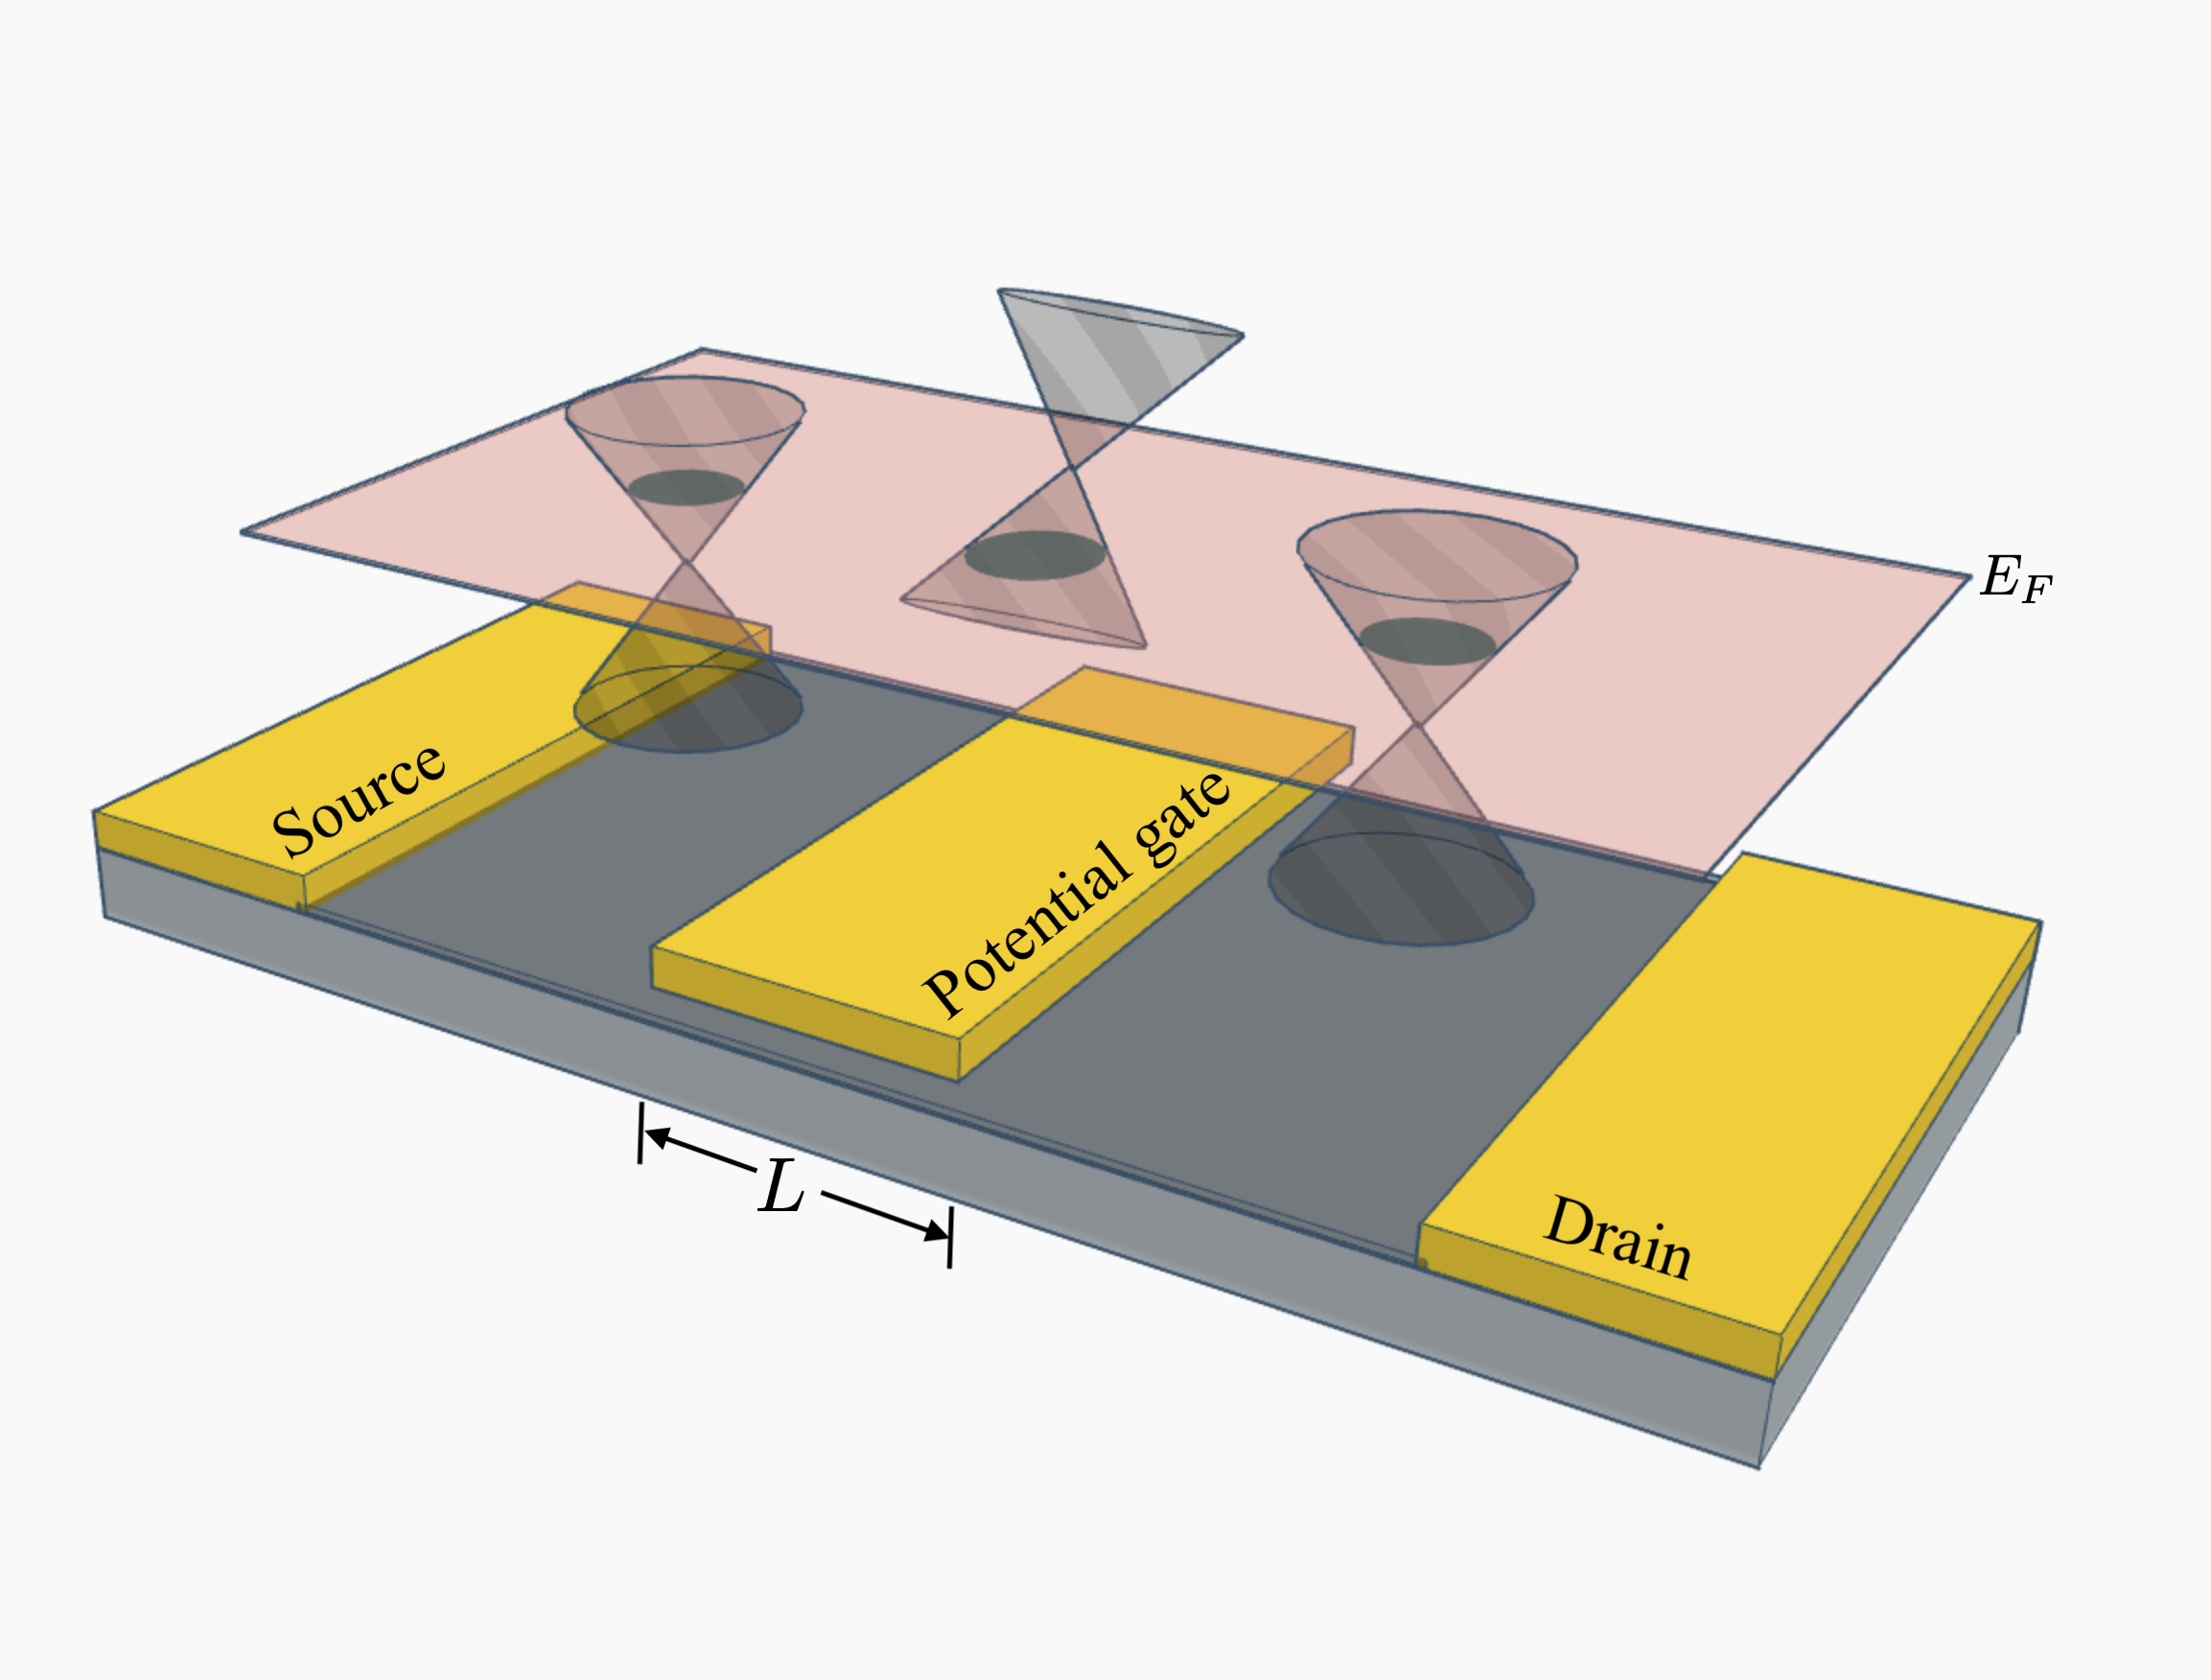
\includegraphics[width=0.6\linewidth]{fig/Transistor.png}
        \caption{Schematic illustration of Dirac material n-p-n heterojunctions with the mismatch of Dirac cone. 
                    The position of Fermi energy level $E_F$ can be controlled by tuning the voltage through potential gate of length $L$.}
        \label{fig:transistor}
    \end{figure}

\section{Transmission probability of electron in tilted Dirac cone}
    The wave function of Dirac electron in general Dirac materials can be obtain by solving the eigenvalue problem.
    Since the low-energy quasiparticles in Dirac material mimic relativistic particle, it can be described by effective massless Dirac Hamiltonian
    \begin{align} \label{eq:Hamiltonian}
        \hat{H} = \hbar (v_F \sigma \cdot k + w \sigma_0 \cdot k) + U \sigma_0
    \end{align}
    where U is barrier height, $v_F=10^6\ \mathrm{ms^{-1}}$ is Fermi velocity, $k=(k_x,k_y)$ is wave vector in the x-y plane, 
    $\sigma=(\sigma_x,\sigma_y)$ is Pauli matrices, $\sigma_0$ is a $2\times2$ identity matrix, 
    and $w=(w_x,w_y)$ is the parameter with the dimension of velocity denoting the tilt of Dirac cone.
    By solving Eq. \ref{eq:Hamiltonian}, we obtain the wave function for each region as follows
    \begin{equation}
    \begin{aligned}
        \psi_1 &= 
        \begin{cases}
            e^{ik_xx} +re^{-ik_xx} \ &, x<0\\
            s(e^{ik_xx}e^{i\phi} +re^{-ik_xx}e^{-i\phi}) \ &, x < 0
        \end{cases}\\
        \psi_2 &=
        \begin{cases}
            ae^{iq_xx} +be^{-iq_xx} \ &, 0\leq x<L\\
            s^\prime(ae^{iq_xx}e^{i\theta} -be^{-iq_xx}e^{-i\theta} )\  &, 0\leq x<L
        \end{cases}\\
        \psi_3 &=
        \begin{cases}
            te^{ik_xx}\ & ,x\geq L\\
            ste^{ik_xx}e^{i\phi}\ & ,x\geq L
        \end{cases}\\
    \end{aligned}
    \end{equation}
    The transmission coefficient $t$ can be obtained by considering the continuity of the wave function at the boundaries $x = 0$ and $x=L$
    \begin{equation} \label{eq:boundary condition}
        \begin{aligned}
            -a-b+r &= -1\\
            -sr e^{-i \phi }-s' \left(a e^{i \theta }-b e^{-i \theta }\right) &= -se^{i \phi }\\
            a e^{i L q_x}+b e^{-i L q_x}-t e^{i k_x L}&=0\\
            s' \left(a e^{i \theta +i L q_x}-b e^{-i \theta -i L q_x}\right)-s t e^{i k_x L+i \phi }&=0\\
        \end{aligned}
    \end{equation}
    It is easier to solve for $t$ using Cramer's rule. First put Eq. \ref{eq:boundary condition} into a matrix form, 
    where each column from left to right contain the factor of the coefficient $r, a, b,$ and $t$ respectively.
    \begin{equation}
        \mathrm{M_1}=
            \begin{pmatrix}
                1 & -1 & -1 & 0 \\
                -s e^{-i \phi } & -s'e^{i \theta } & e^{-i \theta } s' & 0 \\
                0 & e^{i L q_x} & e^{-i L q_x} & -e^{i k_x L} \\
                0 & s' e^{i \theta +i L q_x} & -s' e^{-i \theta -i L q_x} & -s e^{i k_x L+i \phi } \\
            \end{pmatrix}
    \end{equation}
    Then, replace the column $t$ with the factor on the right hand side of Eq. \ref{eq:boundary condition}
    \begin{equation}
        \mathrm{M_2}=
            \begin{pmatrix}
                1 & -1 & -1 & -1 \\
                -s e^{-i \phi } & -s'e^{i \theta }  & e^{-i \theta } s' & -s e^{i \phi } \\
                0 & e^{i L q_x} & e^{-i L q_x} & 0 \\
                0 & s_p e^{i \theta +i L q_x} & -s' e^{-i \theta -i L q_x} & 0 \\
            \end{pmatrix}
    \end{equation}
    The transmission coefficient $t$ can be obtain from $t = \det \mathrm{M_2}/ \det \mathrm{M_1}$
    \begin{equation}
        t = \frac{2 s s' \cos (\theta ) \cos (\phi ) (\sin (k_x L)+i \cos (k_x L))}
        {\sin (L q_x) \left(s^2-2 s s' \sin (\theta ) \sin (\phi )+s'^2\right)+2 i s s' \cos (\theta ) \cos (\phi ) \cos (L q_x)}
    \end{equation}
    The transmission probability can be obtained from $T = t^* t$
    \begin{equation} \label{eq:tp}
        T=\frac{\cos^2 \theta \cos^2 \phi}{\cos^2 (L q_x) \cos^2 \theta \cos^2 \phi + \sin^2 (Lq_x)(1-ss'\sin \theta \sin \phi )^2}
    \end{equation}
\section{The elliptic Fermi surface of tilted Dirac cone} \label{sec:elliptic fermi surface}
    When the Dirac cone is tilted, we obtain the elliptic Fermi surface in which the wavevector of electron is directional-dependent as shown in Fig. \ref{fig:elliptic fermi surface}.
    In other word, the length of vector $k$ varied as it rotate along the elliptic Fermi surface(dashed line).
    To understand relation between the electron wavevector and its incident angle $\phi$, we consider the elliptic equation where the major axis of the ellipse is in y-direction.
    \begin{figure}[H]
        \centering
        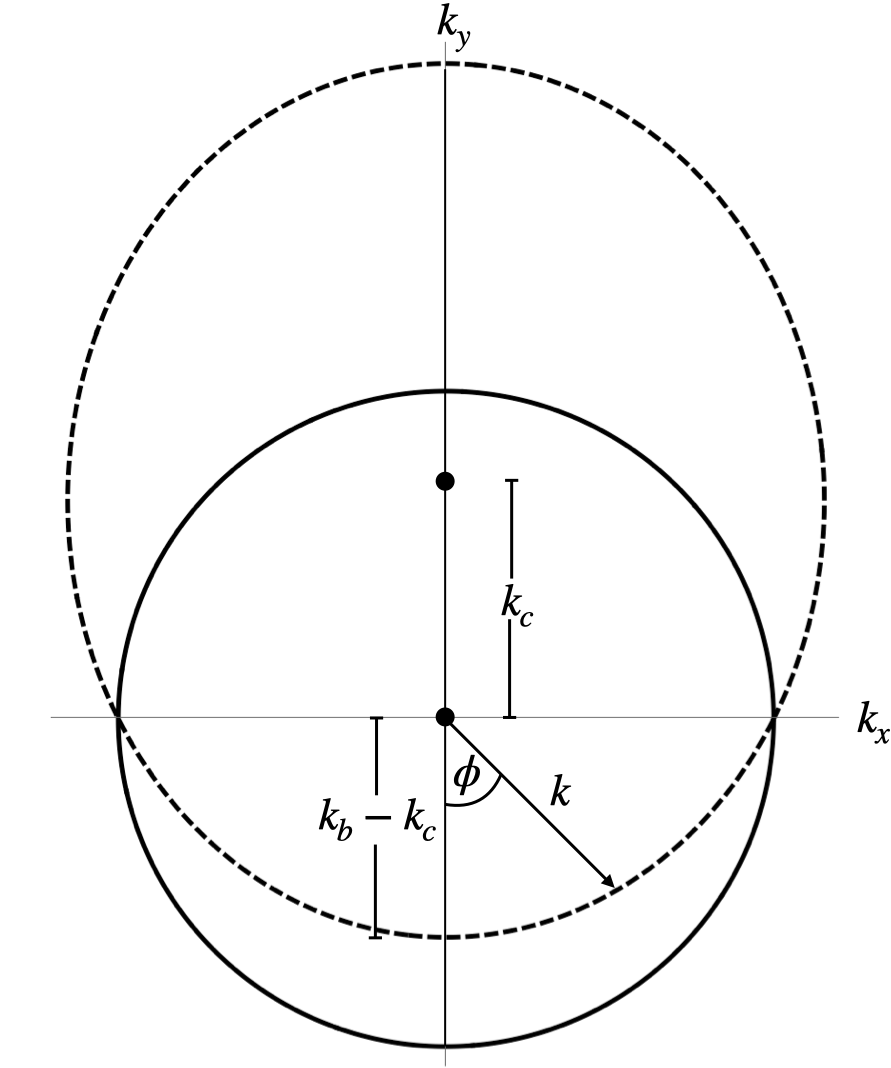
\includegraphics[width = 0.5\linewidth]{fig/elliptic fermi surface.png}
        \caption{The cross-sectional area of non-tilted and tilted Dirac cone with $w_0 = 0.5$ represented by solid and dashed line, respectively.}
        \label{fig:elliptic fermi surface}
    \end{figure}
    \begin{align} \label{eq:elliptic eq}
        \frac{k_x^2}{k_a^2} + \frac{k_y^2}{k_b^2} = 1
    \end{align}
    where $k_x = k\cos{\phi}$ and $k_y = k\sin{\phi} + k_c$. Multiply both side with $k_a^2 k_b^2$ and substituting $\cos^2{\phi} = 1 - \sin^2{\phi}$
    \begin{equation}
        \begin{aligned}
            k_b^2 k^2 -k_b^2 k^2 \sin^2{\phi} + k_a^2k^2 \sin^2{\phi}+2 k_a^2 k c \sin{\phi} +k_a^2 c^2)=k_a^2 k_b^2
        \end{aligned}
    \end{equation}
    Since $k_a = k_b \sqrt{1-w_0^2}$ and $k_c = k_b w_0$ where $w_0$ is eccentricity of the ellipse, we obtain
    \begin{equation}
        \begin{aligned}
            &k_b^2 k^2 - k_b^2 k^2 \sin^2{\phi} + k_b^2 (1-w_0^2)k^2 \sin^2{\phi}\\
            &+2 k_b^2 (1-w_0^2) k k_b w_0 \sin{\phi} +k_b^2 (1-w_0^2) k_b^2 w_0^2=k_b^2 (1-w_0^2) k_b^2\\
        \end{aligned}
    \end{equation}
    Multiplying both side with $-1/k_b^2$ and after some algebra, we obtain
    \begin{align} 
        k = \pm (k w_0 \sin{\phi} - k_b(1-w_0^2))
    \end{align}
    Since $k$ is nonnegative, we have to choose the solution such that $k$ is positive.
    Consider the case where $w_0 = 0$
    $$
    k = \pm (-k_b)
    $$
    We choose the negative solution in order for $k$ to be positive.
    \begin{equation}
    \begin{aligned} \label{eq:k vs phi}
        k &= -k w_0 \sin{\phi}+ k_b (1-w_0^2)\\
        k &= \frac{k_b(1-w_0^2)}{1+w_0 \sin{\phi}}
    \end{aligned}
    \end{equation}

\section{Angular dependent wavevector of tilted Dirac cone} \label{sec:k angular dependent k}
     
    We assume that the Dirac cone only tilted in y-direction. Therefore, the corresponding eigenenergy of Eq. \ref{eq:Hamiltonian} can be written as,
    \begin{align} \label{eq:eigenenergy}
        E_\eta=\hbar (\eta \sqrt{k_x^2 v_x^2+k_y^2 v_y^2 }+k_y w_y)+U
    \end{align}
    where $\eta$ is band index. Since the tilt of Dirac cone determines the shape of Fermi surface in which the wave vector $k$ is directional dependent. 
    In order to see the form of wave vector under the effect of tilted Dirac cone, Eq. \ref{eq:eigenenergy} can be rearranged to elliptic form as
    \begin{align}
        \frac{k_x^2}{k_a^2} + \frac{(k_y+k_c)^2}{k_b^2} = 1
    \end{align}
    where
    $$
    k_a = \frac{(E_F-U) v_y}{\hbar v_x \sqrt{(\eta^2 v_y^2 - w_y^2)} }, k_b = \frac{\eta v_y (E_F-U)}{\hbar (\eta^2 v_y^2 - w_y^2)},
    k_c = \frac{(E_F - U)w_y}{\hbar (\eta^2 v_y^2 - w_y^2)}
    $$
    We have, in section \ref{sec:elliptic fermi surface}, introduced the wavevector of electron as a function of incident angle $\phi$.
    We can substitute $k_b$ and $k_c$ to Eq. \ref{eq:k vs phi}, which gives
    \begin{align} \label{eq:k vs phi final}
        k = \frac{k_b(1-w_0^2)}{1+w_0 \sin{\phi}} = \frac{E_F - U}{\eta \hbar v_F (1+w_0 \sin{\phi})}
    \end{align}
    where
    \begin{equation} \label{3eq: tilted parameter}
        w_0 = \frac{k_c}{k_b} = \frac{(E_F - U)w_y}{\hbar (\eta^2 v_y^2 - w_y^2)} \frac{\hbar (\eta^2 v_y^2 - w_y^2)}{\eta v_y (E_F-U)} = \frac{w_y}{\eta v_F}
    \end{equation} 
    is tilted parameter and $\eta$ is band index indicating that the conduction and valence band always tilted in the opposite direction. 
    Eq. \ref{eq:k vs phi final} is the angular dependent wavevector outside the barrier as a function of incident angle $\phi$.
    Similarly, the wavevector inside the barrier region can be written as
    \begin{equation} \label{eq:q vs theta}
        q = \frac{E_F - U}{\eta \hbar v_F (1+w_0 \sin{\theta})}
    \end{equation}
    where $\theta$ is the refracted angle of electron inside the barrier. 
    This angle depends on the incident angle $\phi$, which can be obtained by considering the conservation of transverse wavevector
    \begin{equation} \label{eq:theta}
        \begin{aligned}
            q_y&=k_y\\
            q\sin{\theta} &= k \sin{\phi}\\
            \theta &= \sin^{-1}\left(\frac{k}{q}{\sin{\phi}}\right).\\
        \end{aligned}
    \end{equation}
    Substitute $\theta$ that we derived above to Eq. \ref{eq:q vs theta}, we obtain
    \begin{equation} \label{eq:q}
        q = \frac{E_F-U}{\hbar v_F s^{\prime}}+\frac{w_0 k_y}{s^{\prime}},
    \end{equation}
    and their x-component can be written as
    \begin{equation} \label{eq:qx}
        \begin{aligned}
        q_x &= \sqrt{q^2-q_y^2}\\
        q_x &= \sqrt{\left(\frac{E_F-U}{\hbar v_F}+w_0 k_y\right)^2-k_y^2}.\\
        \end{aligned}
    \end{equation}

